\section{Simulation Analysis}
\label{sec:simulation}
In this section the steps needed to simulate this circuit using the software Ngspice are described. The analysis (operating point, frequency response and phase response) are the following:
\begin{itemize} 
	\item operating point for $t<0$;
	\item operating point for  $V_s(0) = 0$, replacing the capacitor with a a voltage source $V_x = V_6 - V_8$, where $V_6$ and $V_8$ are the voltages in nodes 6 and 8 as obtained in the previous step (the reason for this is the fact that the equivalent resistance experienced by the capacitor must be calculated. Furthermore, because the energy discharge in the capacitor is continuous, it is required that the initial boundary conditions are computed);
	\item simulate the natural response of the circuit (using the boundary conditions V(6) and V(8) as obtained previously) using a transient analysis;
	\item repeating the third step, using {\it $V_s$} as given in \textbf{equation~\ref{eq:i2}} and f = 1kHz  in order to simulate for the total response on node 6
	\item simulate the frequency response in node 6 for a frequency range 0.1 Hz to 1MHz.
\end{itemize}
\begin {equation}
	v_s( t)  = V_s u(-t) + sin( 2 \pi f t ) u( t)
	\label{eq:i1}
\end{equation}
 with 
\begin {equation}
	u( t ) =  
	\begin{cases*} 
	  0 & if $t < 0$ \\
	1, & if $t \geq 0$
	\end{cases*}
	\label{eq:i31}  
\end{equation}
\pagebreak
%ponto 1
\subsection{Operating Point Analysis for $t<0$}
In this section, there was a need to create a Node 4, between the resistor R6 and Node 7, where an independent voltage source, $V_x$, providing 0V was inserted, to measure the voltage drop ($-V7$) felt by $I_d$. This was created in order to comply with NGSpice's requirements for defining the current controlled voltage source $V_d$.
Table~\ref{tab:op} shows the simulated operating point results for the circuit
under analysis for $t<0$.
%The current flows considered in the theoretical section were coherent with the polarity implicitly declared when defining the circuit to be simulated in the Ngspice script.\par

\begin{table}[H]
  \centering
  \begin{tabular}{|l|r|}
    \hline    
    {\bf Name} & {\bf Value [mA or V]} \\ \hline
    @gb[i] & -2.24128e-04\\ \hline
@id[current] & (  )\\ \hline
@r1[i] & -2.14309e-04\\ \hline
@r2[i] & -2.24128e-04\\ \hline
@r3[i] & -9.81934e-06\\ \hline
@r4[i] & 1.183454e-03\\ \hline
@r5[i] & 1.248524e-03\\ \hline
@r6[i] & -9.69145e-04\\ \hline
@r7[i] & -9.69145e-04\\ \hline
n0 & 4.894946e+00\\ \hline
n1 & -2.98689e+00\\ \hline
n2 & 8.700499e+00\\ \hline
n3 & 4.397911e+00\\ \hline
n4 & 4.864258e+00\\ \hline
n5 & 5.082120e+00\\ \hline
n7 & -2.00234e+00\\ \hline
n8 & -2.00234e+00\\ \hline

  \end{tabular}
  \vspace{10px}
  \caption{Operating point for $t<0$. A variable preceded by @ is of type {\em current}
    and expressed in milliAmpere; other variables are of type {\it voltage} and expressed in
    Volt.}
  \label{tab:op} 
\end{table}
\vspace{9cm}
\pagebreak
%ponto 2

\subsection{Operating Point Analysis for $t=0$}
In this section the circuit is simulated using an operating point analysis with $V_s(0) = 0$ and with the capacitor replaced by a voltage source {\it $V_x=V(6)-V(8)$}, using the values obtained in the last step. This step was taken because we must compute the new initial conditions that guarantee continuity in the capacitor's discharge. Therefore, $V(6) - V(8)$ must be a continuous function, defined in branches (constant for $t<0$ and varying in time for $t \geq 0$), as there can not be a energy discontinuity in the capacitor ($E_C=\frac{1}{2}CV^{2}$). However, that does not imply that that $V(6)$ and $V(8)$ are continuous functions in time.
In \textbf{Table~\ref{tab:opeq}} the simulation results are presented. 
\begin{table}[h!]
  \centering
  \begin{tabular}{|l|r|}
    \hline    
    {\bf Name} & {\bf Value [mA or V and Ohm]} \\ \hline
    \input{opeq_tab}
  \end{tabular} 
  \vspace{10px}
  \caption{Operating point for {\it $v_s(0)=0$}. A variable preceded by @ is of type {\em current}
    and expressed in miliAmpere; variables are of type {\it voltage} and expressed in
    Volt. The equivalent resistance is in Ohms}
  \label{tab:opeq}
\end{table}
\vspace{6cm}
\pagebreak

%ponto 3
\subsection{ Natural solution for $V_6$ using transient analysis}
In this section the natural response of the circuit in the interval [0,20] ms was studied using a transient analysis simulation. Using the previous simulations, the initial conditions for V(6) and V(8) were defined, using NGSpice's diretive \textit{.ic}.
\par


\begin{figure}[H] \centering
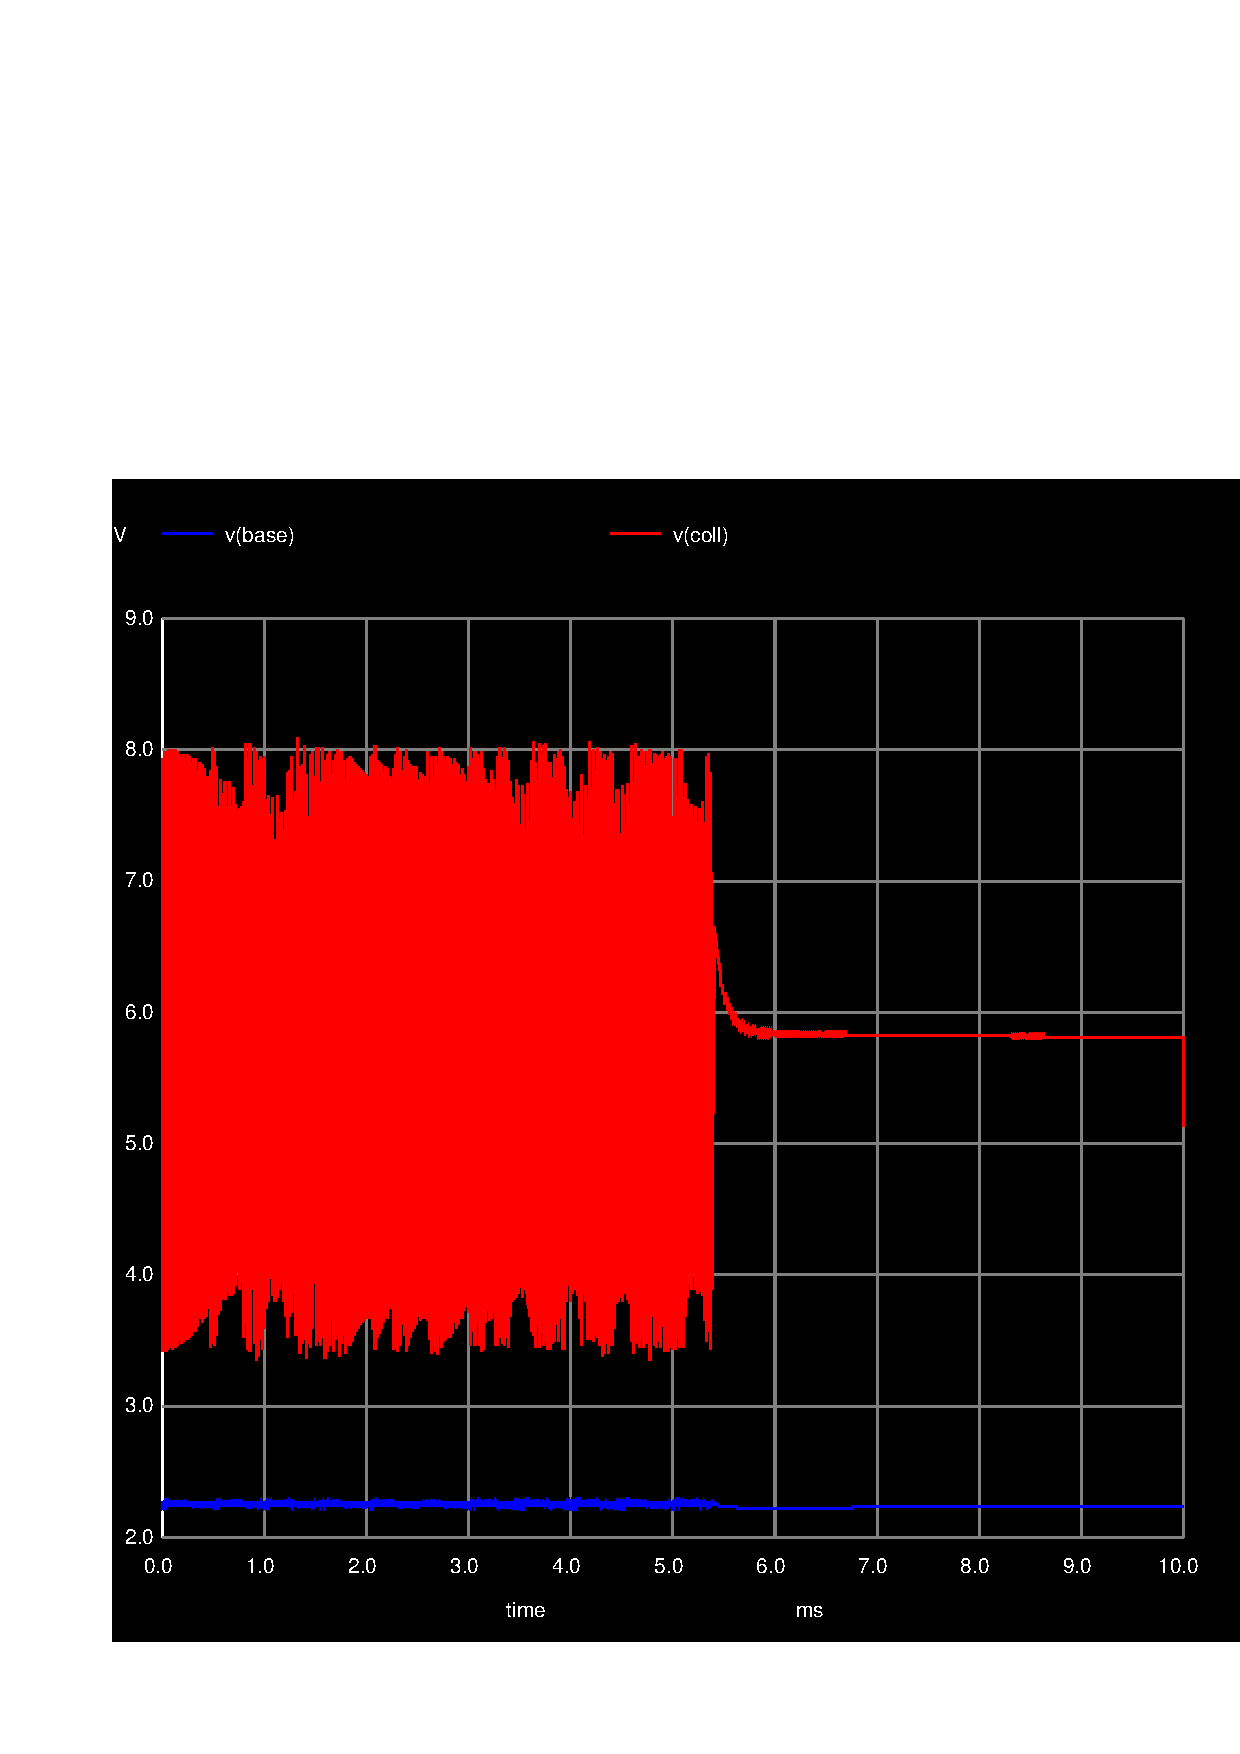
\includegraphics[width=0.7\linewidth]{trans.pdf}
\caption{Simulated natural response of $V_6(t)$ in the interval [0,20] ms. The \textit{x axis} represents the time in milliseconds and the \textit{y axis} the Voltage in node 6  in Volts.  }
\label{fig:transient}
\end{figure}
\vspace{4cm}
\pagebreak
%ponto 4
\subsection{ Total solution for $V_6$ using transient analysis}

In this section the total response of $V_6$ (natural + forced) is simulated using NGSpice's transient analysis capabilities. This is done by repeating the previous section, but using {\it $V_s$} as given in \ref{eq:i2} and f = 1kHz.\par
\begin{figure}[H] \centering
\includegraphics[width=0.6\linewidth]{transv5vs.pdf}
\caption{Simulated response of $V_{6}(t)$ and of the stimulus $V_{s}(t)$ as functions of time from [0,20] ms. The \textit{x axis} represents the time in milliseconds and the \textit{y axis} the Voltage in Volts.}
\label{fig:resp_total}
\end{figure}
\vspace{7cm}
\pagebreak

%ponto 5

\subsection{ Frequency response in node 6}
In this section, the frequency response in node 6 is simulated for the frequency range from 0.1 Hz to 1 MHz, along with the phase response of the circuit.
The reasons of how and why $V_{6}(t)$ and $V_{s}(t)$ differ have been covered in \textbf{subsection ~\ref{ref}}.\par
\begin{figure}[H] \centering
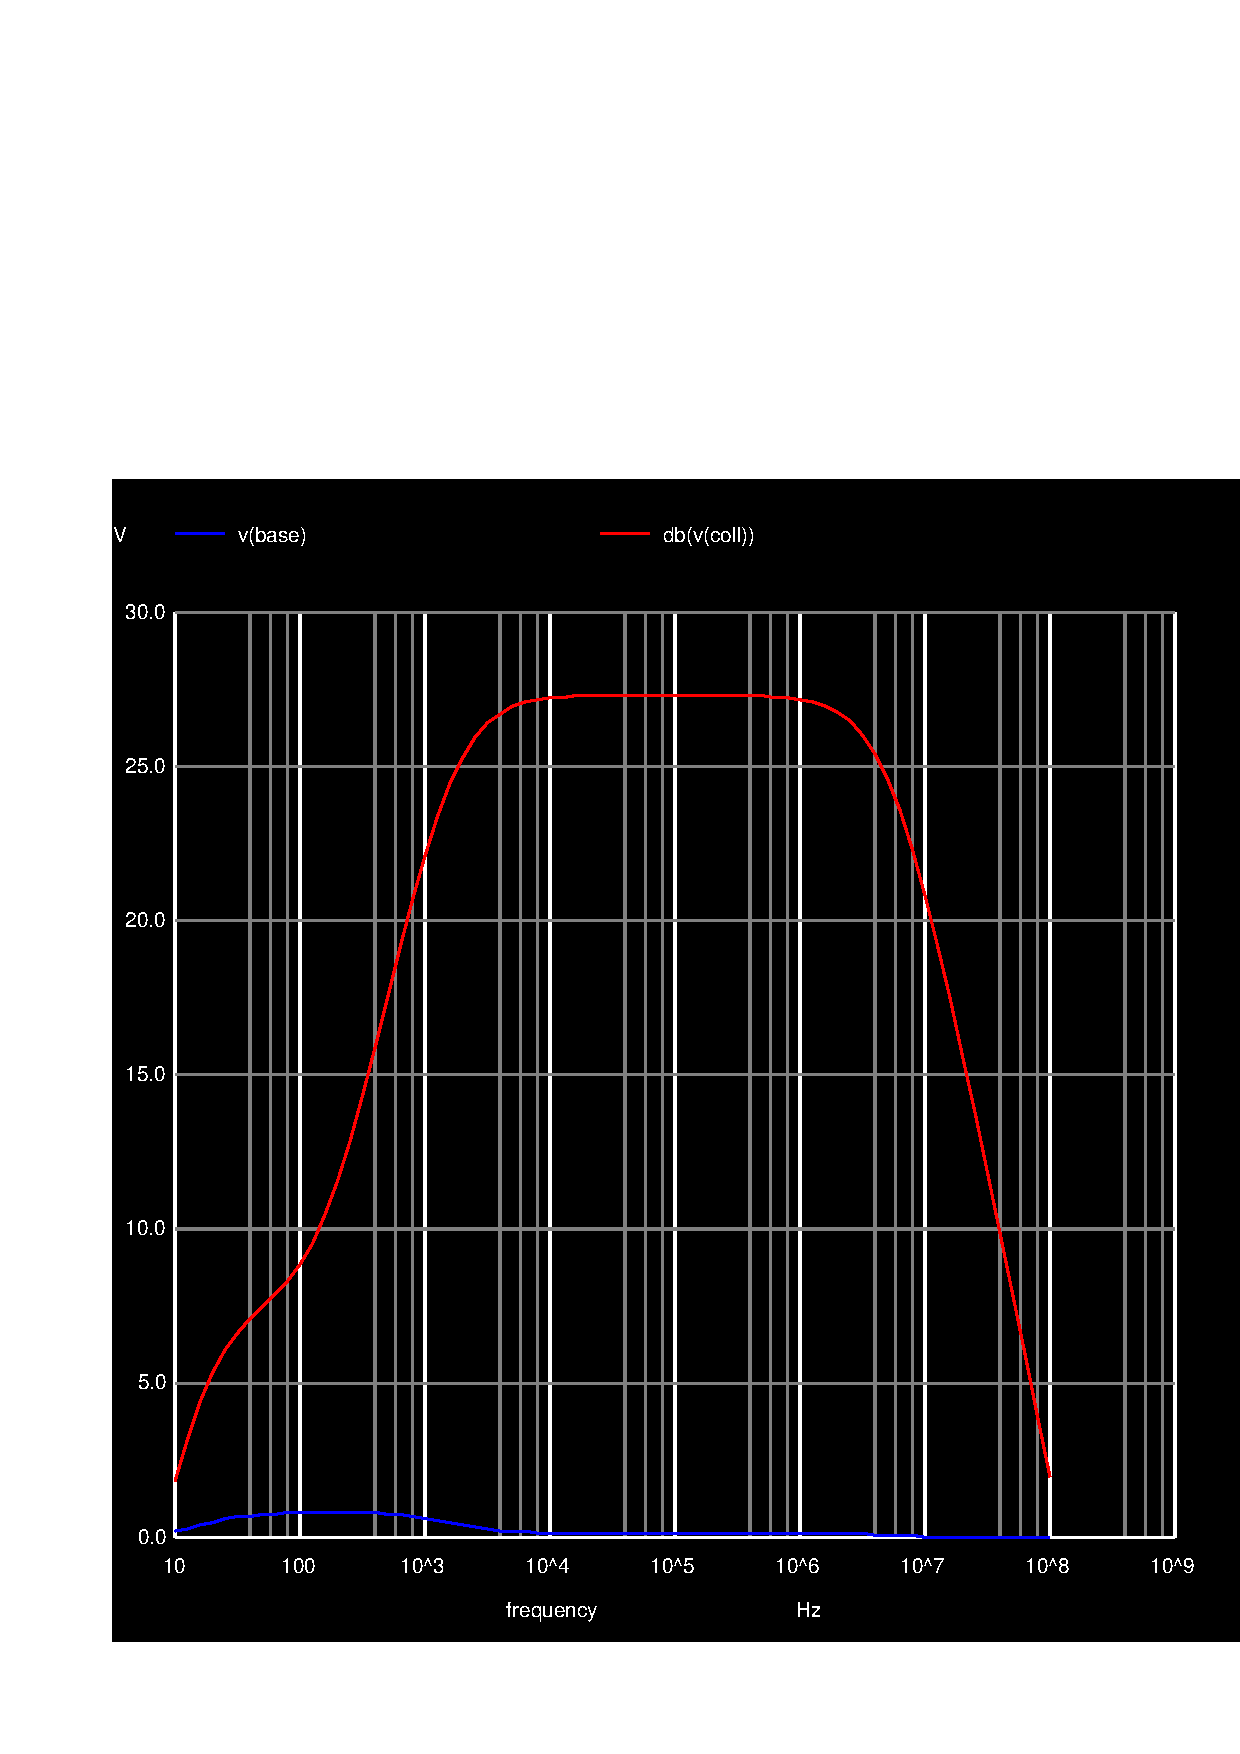
\includegraphics[width=0.4\linewidth]{acm.pdf}
\caption{Magnitude of $V_s(f)$, $V_c(f)$  and of $V_6(f)$. The \textit{x axis} represents the frequency in Hz, using a logarithmic scale and the \textit{y axis} the magnitude in dB.}
\label{fig:Magnitude}
\end{figure}


\par
\begin{figure}[H] \centering
\includegraphics[width=0.4\linewidth]{phase.pdf}
\caption{Phase of $V_s(f)$, $V_c(f)$ and of $V_6(f)$. The \textit{x axis} represents the frequency in HZ, using a logarithmic scale and the \textit{y axis} the phase in degrees.}  
\label{fig:phase}
\end{figure}
